\documentclass[]{article}
\usepackage{amsmath}
\usepackage{amsthm}
\usepackage{amssymb}
\usepackage{graphicx}
\usepackage[utf8]{inputenc} 
\usepackage{subcaption}
\usepackage{caption}
\usepackage{hyperref}
\usepackage{amsbsy}
\usepackage[left=4cm]{geometry}
 %http://tex.stackexchange.com/questions/595/how-can-i-get-bold-math-symbols
%opening
\title{Variance reduction in coarse bifurcation analysis of stochastic models}
\author{Pieter Van Nuffel}

\newcommand{\R}{\ensuremath{\mathbb{R}}} % commando zonder argumenten
\newcommand{\C}{\ensuremath{\mathbb{C}}}
\newcommand{\N}{\ensuremath{\mathbb{N}}}
\newcommand{\E}{\ensuremath{\mathbb{E}}}
\newcommand{\norm}[1]{\left\|#1\right\|} % commando's met argumenten
\newcommand{\pa}[2]{\frac{\partial #1}{\partial #2}}
\newcommand{\ppa}[2]{\frac{\partial^2 #1}{\partial #2^2}}
\newcommand{\dd}{\ensuremath{\mathrm{d}}}
\newcommand{\U}{\ensuremath{\boldsymbol{\rho}}}
\newcommand{\cts}{\ensuremath{\boldsymbol{\Phi}^N_T}} %Coarse time step
\newcommand{\V}{\ensuremath{\mathbf{v}}} 
\newcommand{\jv}{\ensuremath{\mathbf{\hat{Jv}}}}
\newcommand{\jvpde}{\ensuremath{\mathbf{Jv}_{FP}}}

\theoremstyle{definition}
\newtheorem{Theorem}{Theorem}


\begin{document}-



 
\section{Model problem}



%
%We investigate coarse equilibrium states of a stochastic model 
%
%
% we derive an analytic
%approximate coarse evolution-map for the expected average purchase. We then study the emergence
%of coarse fronts when the agents are split into two factions with opposite preferences. We
%develop a novel Newton-Krylov method that is able to compute accurately and efficiently coarse
%fixed points when the underlying fine-scale dynamics is stochastic. The main novelty of the algorithm
%is in the elimination of the noise that is generated when estimating Jacobian-vector products
%using time-integration of perturbed initial conditions. We present numerical results that demonstrate
%the convergence properties of the numerical method, and use the method to show that macroscopic
%fronts in this model destabilise at a coarse symmetry-breaking bifurcation.
%
%We consider a system of diffusion processes that interact through their empirical mean and have a stabilizing force acting on each of them, corresponding to a bistable potential. There are three parameters that characterize the system: the strength of the intrinsic stabilization, the strength of the external random perturbations, and the degree of cooperation or interaction between them. The latter is the rate of mean reversion of each component to the empirical mean of the system. We interpret this model in the context of systemic risk and analyze in detail the effect of cooperation between the components, that is, the rate of mean reversion. We show that in a certain regime of parameters increasing cooperation tends to increase the stability of the individual agents but it also increases the overall or systemic risk. We use the theory of large deviations of diffusions interacting through their mean field.
%
%
%The present paper thus contains two main contributions. First, for the specific
%system under study, we explain the birth of the above-described macroscopic states in
%terms of coarse symmetry-breaking bifurcations. To the best of our knowledge, steps
%in this direction were taken only very recently [55, 7] and were confined to globally
%locked-in states. In the homogeneous case, we follow [5] and interpret metastable
%locked-in states as fixed points of a coarse evolution map. In the limit of infinitely
%many globally-coupled agents with homogeneous product preferences, we derive the
%coarse evolution map analytically. In the case of heterogeneous agents we employ
%stochastic continuation and show for the first time how fronts destabilise to partially
%locked-in states.
%The second main contribution of the paper is the development of a novel procedure
%to obtain coarse Jacobian-vector products with reduced variance, allowing
%the accurate evaluation of Jacobian-vector products in the presence of microscopic
%stochasticity, thus gaining full control over the linear and the nonlinear iterations
%of the Newton-Krylov solver. Even though our implementation of variance-reduced
%Jacobian-vector products is specific to the lock-in model, we believe that analogous
%strategies can be applied to other ABMs. Therefore, we provide a detailed account of
%the algorithmic steps involved in defining anf accurate equation-free Newton-Krylov
%method and testing its convergence properties


%\section{Systemic risk}

Until now, we considered a system of non-interacting particles. We will now extend our model to a mean field model by introducing a third parameter $\alpha$, which is the degree of interaction or cooperation in the system. A simple form of cooperative behaviour is the case where each agent tends to follow the state of the majority (or, each particle feels an attractive force towards the mean state of the system). To include this cooperation effect in our stochastic simulation, we add this mean reversion term to the SDE \eqref{SDE}:

\begin{equation} 
\label{SDE_meanfield}
    \dd x = \mu V(x) \dd t + \sigma  \dd{W_t} + \alpha(\bar{x} -x) \dd t ,
\end{equation}
with  $\bar{x}(t) = \frac{1}{N} \sum_{i=1}^{N} x_i(t)$ denoting the empirical mean. 


An interesting application of this model to banks and insurance is the emergence of systemic risk.  Banks will try to minimize their own individual risk by spreading the risk between each other. However, this may increase the risk that they may all fail: reducing individual risk on a micro-scale can increase systemic risk on a macro-scale. 
Garnier, Papanicolaou and Yang already made use of the dynamics in eq. \eqref{SDE_meanfield}  to show that interconnectedness between agents indeed affects the stability of the whole system, causing systemic risk  \cite{Garnier}. They defined $x_i$  as the state of risk of agent $i$. The bi-stable-state structure of the potential $V(x)$ ensures that each risk variable stays around $-1$ (defined as the normal state) or $+1$ (the failed state).  A natural measure of systemic risk is then the transition probability of the empirical mean $\bar{x}$ from the normal state to the failed state. 
 

To establish the idea, let us repeat the numerical simulations with eq. \ref{SDE_meanfield}. The evolution of the system is now characterized by  by the initial conditions, the three parameters ($\mu$, $\sigma$, $\alpha$) and by the system size $N$. Figure \ref{fig:sysrisk}  illustrates the behaviour of the empirical mean $\bar{x}$. The simulations were performed with all agents initially in the normal state. Nevertheless, if randomness dominates the interaction, the agents can move immediately to the other potential well. The system then behaves like $N$ independent diffusions, and hence, by the symmetry of the potential, the mean state will be attracted to a single mixed state $\bar{x}=0$. Upon increasing the interaction parameter $\alpha$, however, we find two new macroscopic states, suggesting the presence of a pitchfork bifurcation at the macroscopic level. These solutions are no stable steady states, but rather coarse metastable states. Their lifetime is linked to the finite system size. 



\begin{center}
\begin{figure}
\includegraphics[width=0.5\textwidth]{../../riskmodel/Problems/WeightedParticles/checkSystem/plots/xmean_alpha1}
\includegraphics[width=0.5\textwidth]{../../riskmodel/Problems/WeightedParticles/checkSystem/plots/xmean_alpha5}

\caption{The empirical mean, simulated for different $\alpha$. \textit{Left}: the system has one single state $\bar{x}=0$. \textit{Right}: for $\alpha> \alpha_c$ two metastable equilibria emerge. 
 The red dashed lines are approximated  analytical solutions for the steady states. \label{fig:sysrisk}}
\end{figure}
\end{center}


 \begin{center}
\begin{table}
\caption{Parameter values}
  \begin{tabular} { | c  c | c |}    \hline   
     %FTCS-scheme  &   Euler-Maruyama-scheme  \\  
   \textit{ {Discretization parameters}}&    &  SDE    \\ \hline
    Discretization step  & $\Delta x $  & $10^{-2}$ \\ 
        Number of discretization steps  & $n_x$ &  340 \\ 
    Time step  &  $\Delta t$ &   $10^{-2}$ \\ 
       Number of timesteps  & $n$  &  $10^{6}$ \\ \hline
  \end{tabular}
%\quad
%     \begin{tabular}  { | c | c | c |  }  \hline
%     \multicolumn{3}{|c|} {\textit{ System parameters}   }    \\
%    \hline  
%    Diffusion coefficient  & $D $ & $0.5$ \\ 
%   Drift coefficient &  $\mu$ & $ 1$ \\ \hline
%  \end{tabular}
\end{table}
\end{center}



\subsubsection{Calculating fixed points}
The steady  states are computed with the Newton-Krylov solver described in section \ref{sec:Newton-Krylov} and compared with the approximated analytical solutions, calculated by Garnier et. al for small $h$ \cite{Garnier}.


\begin{center}
\begin{figure}
\includegraphics[width=1\textwidth]{../../riskmodel/Problems/WeightedParticles/checkSystem/plots/steady_states.pdf}
\caption{\label{fig:bif_anal}}
\end{figure}
\end{center}



\subsubsection{Continuation}
We use a pseudo-arclength contunaution method with secant prediction steps.
In fig. \ref{todo} we show a bifurcation diagram of the densities. 





\begin{center}
\begin{figure}
\includegraphics[width=0.8\textwidth]{../../riskmodel/Problems/WeightedParticles/checkSystem/plots/bif_alpha}
\caption{\label{fig:bif_anal}}
\end{figure}
\end{center}






By adding the mean reversion term, the Fokker-Planck equation \eqref{fokkerplanck}  describing the evolution of the density, now becomes

\begin{equation}
\label{fp_mean_field}
\pa{\rho(x,t)}{t} = - \mu \pa{( f(x) \rho(x,t))}{x} - \alpha \pa{}{x} \left[ \left(\int x \rho(x,t) \mathrm{d}x  -x \right) \rho(x,t) \right] + \frac{\sigma^2}{2}  \ppa{\rho(x,t)}{x} .
\end{equation}

Explicit solutions of eq. \label{fp_mean_field} are not available in general, but we can find equilibrium solutions. Assuming that \(\xi = \lim_{t \to \infty} \int x \rho(x,t) \mathrm{d}x \), an equilibrium solution satisfies
\begin{equation}
\mu \pa{( f(x) \rho_{\xi}) }{x}   - \alpha \pa{}{x} \left [( \xi -x) \rho_{\xi}  \right] +\frac{\sigma^2}{2} \ppa{\rho_{\xi}}{x}
\end{equation}
 -
and has the form 
\begin{equation}
\rho_{\xi}(x) = \frac{1} {Z_{\xi}} \exp{ \left( -\frac{(y-\xi)^2}{2 \frac{\sigma^2}{2 \alpha}} - \mu \frac{2}{\sigma^2} V(x)  \right)}
\end{equation}
In addition, the non-zero solutions $\pm\xi$ are


\begin{equation}
\xi = \pm \sqrt{1-3\frac{\sigma^2}{2\theta}}\left(1+
\ \mu \frac{6}{\sigma^2}\left(\frac{\sigma^2}{2\theta}\right)^2\frac{1-2\frac{\sigma^2}{2\theta} }{1-3\frac{\sigma^2}{2\theta}}\right) + \mathcal{O}(\mu^2)
\end{equation}  




%\begin{equation}
%\label{fokkerplanck}
%\pa{\rho(x,t)}{t} = - \mu \pa{( U(x) \rho(x,t))}{x} - \alpha \pa{}{x} \left[ \left(\int x \rho(x,t) \mathrm{d}x  -x \right) \rho(x,t) \right] + D  \ppa{\rho(x,t)}{x} 
%\end{equation}\mathrm{d}x



%
%\begin{figure}
%\includegraphics{../../riskmodel/Problems/WeightedParticles/checkSystem/plots/xmean_alpha5}
%
%\end{figure}


\begin{figure}
\centering
\includegraphics[width=0.49\linewidth]{/home/pieter/riskmodel/Problems/WeightedParticles/checkSystem/plots/Newton_states_abs_bias_N1e6}
\includegraphics[width=0.49\linewidth]{/home/pieter/riskmodel/Problems/WeightedParticles/checkSystem/plots/Newton_states_abs_bias_N1e4_5_6_7}
\caption{The bias between the analytical solution $\xi$ and the mean $\bar{x}$ of the density calculated with the Newton-Krylov solver is plotted as a function of the number of Newton iterations $k$. This bias converges to zero with a rate depending on the timestep used in the coarse time stepper $\Delta T$, but not on the number of particles $N$.  ($\Delta x = 10^{-2}$, $\Delta t = 10^{-2}$, $\mu=0.05$, $\alpha=5$, $\sigma=1$)}
\label{fig:Newton_states_bias_mean}
\end{figure}

%\begin{figure}
%\centering
%\includegraphics[width=0.49\linewidth]{/home/pieter/riskmodel/Problems/WeightedParticles/checkSystem/plots/Newton_states_abs_bias_N1e4_5_6_7_log}
%\includegraphics[width=0.49\linewidth]{/home/pieter/riskmodel/Problems/WeightedParticles/checkSystem/plots/bias_steady_states_f(Dt)}
%\caption{Is the total number of timesteps used in the Newton-Krylov-method (\textit{left}) significantly lower than the number of timesteps used in direct simulation (\textit{right}) to reach the same accuracy? Not clear from these plots}
%\label{fig:bias_steady_states_f(Dt)}
%\end{figure}
%

\begin{figure}
\centering
\includegraphics[width=0.7\linewidth]{/home/pieter/riskmodel/Problems/WeightedParticles/checkSystem/plots/bias_compare_Newton_direct}
\caption{The total number of timesteps used in the Newton-Krylov-method is lower than the number of timesteps  in direct simulation to calculate a fixed point with the same accuracy. ($N=10^6$,$\Delta x = 10^{-2}$, $\Delta t = 10^{-2}$, $\mu=0.05$, $\alpha=5$, $\sigma=1$) }
\label{fig:bias_compare_Newton_direct}
\end{figure}

\begin{figure}
\centering
\includegraphics[width=0.49\linewidth]{/home/pieter/riskmodel/Problems/WeightedParticles/checkSystem/plots/res_norm_gmres_e-5_alpha5_mu0p05}
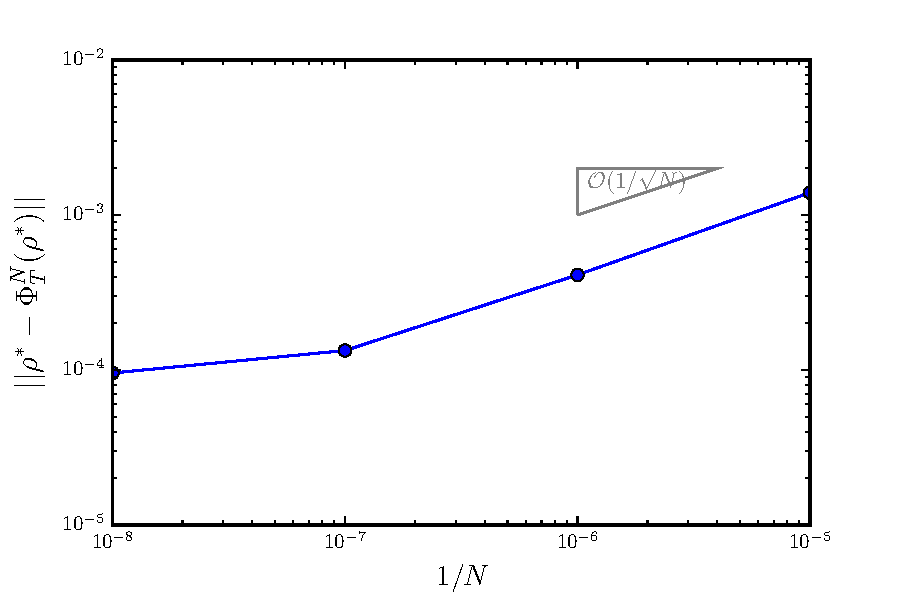
\includegraphics[width=0.49\linewidth]{/home/pieter/riskmodel/Problems/WeightedParticles/checkSystem/plots/Tolerance_on_NK-solution_converges_N-1}
\caption{The needed number of Newton iterations and the tolerance after convergence depend on the number of particles $N$ (\textit{left}). This best achieved tolerance converges to zero with  $\mathcal{O}(\frac{1}{\sqrt{N}})$ (\textit{right}). (Parameter values: $\Delta x = 10^{-2}$, $\Delta t = 10^{-2}$, $\Delta T = 10 $ $\mu=0.05$, $\alpha=5$, $\sigma=1$, $ \epsilon_{\texttt{GMRES}}=10^{-5}$)}
\label{fig:Tolerance_on_NK-solution_converges_N-1}
\end{figure}

\begin{figure}
\centering
\includegraphics[width=0.7\linewidth]{/home/pieter/riskmodel/Problems/WeightedParticles/checkSystem/plots/bifurcation}
\caption{}
\label{fig:bifurcation}
\end{figure}








%
%\bibliographystyle{plain}
%\bibliography{biblio.bib}





\end{document}
